\section{Hellfire and COMPaaS Integration Layer (HAC)}
\label{sec:HAC}
Como objetivo deste trabalho, temos a criação de uma camada de integração entre o sistema de tempo real
, previamente descrito, HellfireOS~\ref{HellfireOS} e a plataforma COMPaaS, também analisada anteriormente~\ref{COMPaaS}.
Essa camada consistirá em adicionar suporte a duas questões críticas no HellfireOS, uma biblioteca compatível
com o protocolo de comunicação esperado pela camada de mais baixo nível do COMPaaS e, para prova de conceito,
uma meio de comunicação entre o HellfireOS e a plataforma IoT, tendo em vista que o sistema operacional
ainda não possui uma implementação de todas as camadas de rede necessárias, como por exemplo, o protocolo
TCP.

\begin{figure}[H]
	\centering
		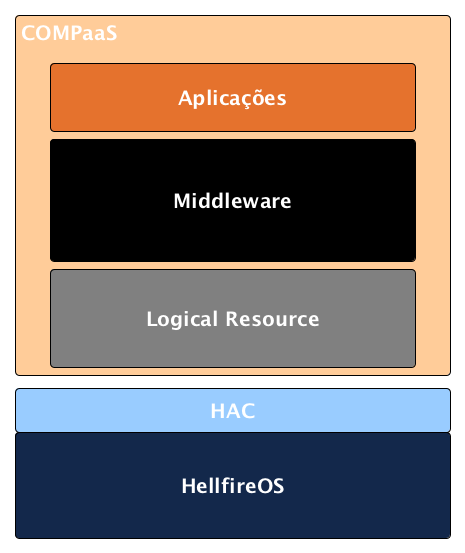
\includegraphics[width=0.3\textwidth]{fig/COMPaaS_HF.png}
	\caption{Arquitetura em alto nível da integração com a camada de integração.}
\end{figure}

Para fins de validação da camada de integração, será criado um protótipo utilizadando uma placa
CubieBoard rodando um sistema Linux que rodará o sistema HellfireOS virtualizado. O meio de comunicação
entre o host Linux e o HellfireOS será feito através de um espaço de memória compartilhada, que será
abstraída da camada de integração desenvolvida, permitindo que a mesma camada seja utilizada com
poucas ou nenhuma alteração quando o HellfireOS possuir outros meios de comunicação via rede.
Para possibilitar que essa comunicação entre host e HellfireOS funcione, será desenvolvida uma
daemon no sistema host para interfacear sua camada de comunicação via rede com a comunicação
via memória compartilhada com o sistema de tempo real.

\subsection{Prova de Conceito}
Para provar a o funcionamento da camada de integração, será utilizada uma
simulação de sensor médico baseado em funções matemáticas suportadas pelo HellfireOS
ou mesmo um sensor real, caso haja o suporte Cubieboard, HellfireOS e sensor disponível.
